\section{Hadoop}
\subsection{Breve histórico}
O problema era simples: como criar um índice para uma máquina de busca de toda a Internet? Foi com esse desafio que Mike Cafarella e Doug Cutting resolveram desenvolver o Apache Nutch. Rapidamente o \textit{crawler} e a máquina de busca ficaram prontos, mas eles perceberam que a arquitetura não escalaria para criar um índice de mais de um bilhão de páginas da Internet. Na mesma época, a equipe do Google publicou um conhecido artigo que explicava a arquitetura do GFS (Google FileSystem) \cite{ghemawat2003google}, que era um sistema de arquivos distribuído que era usado em sua máquina de busca. Doug e Mike decidiram criar uma implementação \textit{open source} dessa arquitetura e a chamaram de NDFS (Nutch Distributed FileSystem).

Em 2004, a equipe do Google publicou um artigo detalhando como era possível criar um índice de toda a Internet usando um conceito denominado MapReduce \cite{dean2008mapreduce}. Com base nesse trabalho, os desenvolvedores do Nutch migraram a maior parte de seus algoritmos para executar sobre o MapReduce e o NDFS. Mais tarde, Doug Cutting foi trabalhar no Yahoo! liderando uma equipe que construiu a nova geração de máquina de busca deles. Depois, o NDFS e o MapReduce tornaram-se um projeto da Apache sob o nome de Apache Hadoop.

Desde então, o Hadoop tem sido usado mundialmente para processar enormes quantidades de dados. Vários frameworks foram construídos para executar usando a sua infraestrutura, como veremos a seguir. Diversos fornecedores criaram suas próprias distribuições do Hadoop, como Microsoft, IBM, EMC, Oracle e outras empresas especializadas como Cloudera e Hortonworks.

\subsection{Funcionamento do HDFS}
O HDFS, como mencionado acima, é um sistema de arquivos distribuídos, projetado para armazenar arquivos muito grandes\footnote{Atualmente há instâncias do HDFS armazenando PetaBytes de dados.} executando sobre \textit{hardware} barato. 

Assim como em qualquer sistema de arquivos, um arquivo é dividido em \textbf{blocos} de dados. Enquanto, tipicamente um sistema de arquivos tradicional armazena dados em blocos de 512 bytes, o HDFS usa, por padrão, blocos de 64MB. Isso torna o HDFS ineficiente para uso em arquivos muito pequenos e numerosos. Para garantir disponibilidade e leitura em paralelo, cada um dos blocos é replicado em um dos nós de um \textit{cluster} HDFS. Quando um disco ou um dos nós do \textit{cluster} falha, além do bloco poder ser lido de outro nó, o sistema de arquivos automaticamente recria os blocos presentes naquele disco em outros nós do \textit{cluster}.
\begin{figure}
	\centering
	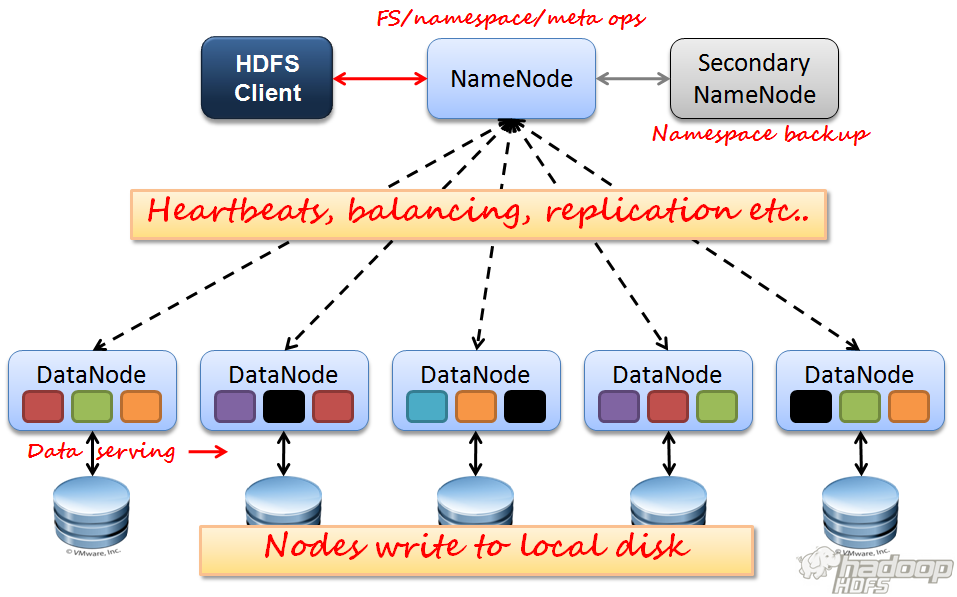
\includegraphics[width=\linewidth]{./hdfs_architecture.png}
	\caption{Visão geral da arquitetura do HDFS}
	\label{fig:hdfs_arch}
\end{figure}

A arquitetura de um \textit{cluster} HDFS divide-se em \textit{NameNode} e \textit{DataNode}. O primeiro armazena um índice de arquivos e de seus blocos e o segundo armazena os dados (blocos). Um cliente que queira ler arquivos no HDFS, primeiro consulta o \textit{NameNode}, que então diz de quais nós do cluster os blocos serão lidos, garantindo um balanceamento de carga na leitura. Arquivos criados no HDFS só podem ser modificados anexando conteúdo no final. Não pode-se modificar blocos já escritos. A falha do \textit{DataNode} implica na indisponibilidade de todo o HDFS e, por esse motivo, é importante mantê-lo resiliente a falha com mecanismos de redundância. Uma visão geral dessa arquitetura pode ser vista na figura \ref{fig:hdfs_arch}.

\subsection{O ecossistema Hadoop}
Atualmente o Hadoop conta com um ecossistema com diversos \textit{frameworks}. Uma lista, não exaustiva, de alguns dos principais projetos que compõem o ecossistema pode ser vista abaixo.
\begin{itemize}
	\item Ambari: Uma ferramenta web para aprovisionamento e gerenciamento de um cluster Hadoop e de diversos de seus componentes.
	\item HBase: Um banco de dados relacional e colunar que utiliza a infraestrutura do Hadoop como mecanismo de armazenamento.
	\item Hive: Uma infraestrutura de armazém de dados com suporte a sumarização de dados e consultas.
	\item Pig: Uma linguagem de alto nível para fluxo de dados e um \textit{framework} de execução de computação distribuída. 
	\item Spark: Uma \textit{engine} rápida e de propósito geral para processamento de dados em memória baseados nos dados do HDFS. O Spark oferece um modelo de programação simples e poderoso para executar uma enorme gama de atividades como ETL, aprendizagem de máquina, processamento contínuo de dados, processamento de grafos, etc.
	\item Sqoop: uma ferramenta para transferência massiva de dados entre bancos de dados relacionais e o HDFS.
	\item Mahout: Um conjunto de bibliotecas para executar algoritmos de aprendizagem de máquina e mineração de dados. Os coordenadores do projeto decidiram mover a implementação dos algoritmos de MapReduce para o Spark.
\end{itemize}

\subsection{MapReduce}
O Hadoop MapReduce é um \textit{framework} para facilitar a escrita de programas de computador para processar uma enorme quantidade de dados de forma paralela, distribuída e resiliente a falhas. Os dados de entrada para um \textit{Job} MapReduce, por estarem armazenados no HDFS, são também processados de forma distribuída, aproveitando dos dados disponíveis localmente em um nó do \textit{cluster}. Na \ref{fig:mapreduce} podemos ver um desenho esquemático de um \textit{Job} MapReduce, que  é, de forma resumida, composto por duas fases:
\begin{enumerate}
	\item Map - quando os dados são processados e produzem saídas como tuplas no formato (Chave, Valor); 
	\item Reduce - quando as tuplas com mesma chave são agrupadas para alguma atividade de agregação.  
\end{enumerate}

\begin{figure}
	\centering
	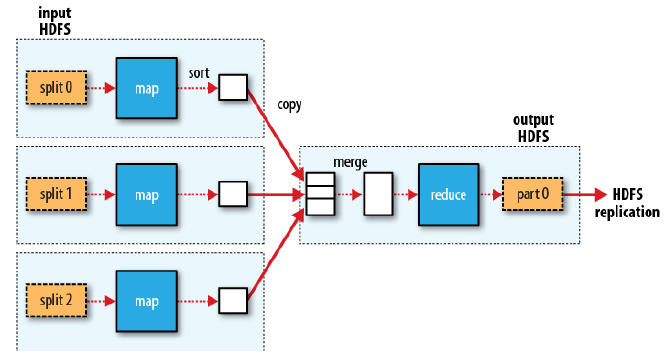
\includegraphics[width=\linewidth]{./mapreduce_job.png}
	\caption{Um \textit{Job} MapReduce}
	\label{fig:mapreduce}
\end{figure}

Um exemplo bem simples para entender o MapReduce é um Job para contar a ocorrência de cada palavra em um texto. Na fase de Map, cada linha lida do arquivo é dividida em suas palavras que produzem uma saída (PalavraA, 1). Note que se uma palavra aparece duas vezes na mesma linha duas tuplas idênticas serão produzidas. Na faze de Reduce, as tuplas com mesma chave serão agrupadas e os valores serão somados. 

Em geral, o programador não precisa se preocupar com comunicação de dados, tratamento de concorrência e eventuais falhas em algum nó que está processando um determinado \textit{Job}. Esse é um dos grandes diferenciais do Hadoop MapReduce. 

\subsection{Pig}
nessa seção vou explicar o mapreduce e como resolver o problema do triangulo

\section{Apache Spark}
O Apache Spark é uma plataforma para computação distribuída que foi projetada para ser de propósito geral e muito eficiente \cite{karau2015learning}. A principal diferença em relação ao MapReduce é que toda a computação é feita e armazenada em memória, sem necessidade de salvar em disco resultados intermediários. 

A unidade básica de dados do Spark é o \textit{Resilient Distributed Dataset} (RDD). O conceito é semelhante ao bloco de dados do HDFS, mas trata-se de coleções de dados que estão na memória RAM dos nós do \textit{cluster}. Na prática, o Spark carrega os dados de um bloco do HDFS na memória RAM do nó em que o bloco está. Os programas Spark fazem dois tipos de operação com um RDD:
\begin{itemize}
	\item \textbf{Transformações}: Transformam um RDD em outro RDD. Entre as transformações mais comuns podemos encontrar as operações de Map e ReduceByKey (mesmo conceito do MapReduce), ordenação e operações de conjuntos, como união, interseção e diferença.
	\item \textbf{Ações}: Produzem algum resultado a partir de um RDD. Ações típicas consistem em enumerar alguma quantidade de itens de um RDD, contar e somar. 
\end{itemize}

O Spark utiliza o conceito de "execução preguiçosa", para que só quando realmente um resultado tenha de ser produzido (uma \textbf{ação} é executada), e toda a sequência de passos necessária é conhecida, o Spark realmente lê os dados e faz cálculos na memória. Com isso, o motor de execução do Spark consegue otimizar tudo que será executado, escolhendo os melhores nós, a melhor sequência, etc.

O Apache Spark também vem com um conjunto de bibliotecas com algoritmos para aprendizado de máquina, grafos, fluxo contínuo de dados e SQL. Algumas dessas vermos a seguir.

\subsection{Utilizando o console python}
O Apache Spark possui consoles iterativos nas linguagens Python e Scala e seus \textit{Jobs} podem ser submetidos em batch também em Java. A API do Spark é acessada a partir de um objeto central denominado \texttt{ SparkContext }. Esse objeto contém a conexão com uma instância do cluster e a partir dele todos os outros objetos e métodos são acessados. Ao se iniciar um console do Spark, o objeto já está automaticamente disponível através da variável \texttt{ sc }. Para compreender a simplicidade do modelo de programação do Spark, o trecho de código abaixo lê um arquivo txt e faz a contagem de ocorrência das palavras.

\begin{lstlisting}[style=MyPythonStyle]
#produz um RDD onde cada item e uma linha do arquivo texto
arquivo = sc.textFile('hdfs://servidor:10001/arquivo.txt') 

#para cada linha produz N itens no novo RDD, uma para cada palavra.
palavras = arquivo.flatMap(lambda linha : linha.split(' ')) 

#cria novo RDD com tuplas do formato (palavra, 1)
palavrasCV = palavras.map(lambda palavra : (palavra, 1)) 

#executa o Reduce usando a funcaoo add para os valores das tuplas.
contagemPalafras = palavrasCV.reduceByKey(add) 

#somente nesse comando toda a computacaoo e feita de forma otimizada.
contagemPalavras.collect() 
\end{lstlisting}

Para resolver o problema de contagem de triângulos utilizando o Spark, a idéia é semelhante à usada com o modelo do MapReduce.

\subsection{Spark SQL}
O Spark SQL é um módulo do Apache Spark para processamento de dados estruturados (relacionais). Ele utiliza uma abstração denominada DataFrame, e também serve como uma máquina de execução de consultas distribuídas baseada em SQL. 

Um DataFrame do Spark SQL tem as mesmas características de um DataFrame em R ou em Pandas (Python) e pode ser criado baseando-se em diversas fontes de dados, como um arquivo json, um arquivo texto, um RDD do Spark, uma tabela do Hive, ou qualquer fonte que possua um driver JDBC. O \textit{schema} de um DataFrame pode ser inferido através de reflexão ou definido programaticamente. 

O trecho de código abaixo mostra como executar a contagem de triângulos utilizando o SQL proposto na seção \ref{triangulos}.

\begin{lstlisting}[style=MyPythonStyle]
# Importa os modulos e cria o contexto
from pyspark.sql import SQLContext, Row
sqlContext = SQLContext(sc)

# Carrega o arquivo de arestas para um RDD
linhas = sc.textFile("hdfs://npaa0352:10001/data/triangles/twitter_combined.txt")
partes = linhas.map(lambda l: l.split())
arestas = partes.map(lambda p: Row(follower=int(p[0]), followee=int(p[1])))

# Infere o schema e registra o DataFrame como tabela
schemaWiki = sqlContext.createDataFrame(arestas)
schemaWiki.registerTempTable("arestas")

# Executa o SQL
triangulos = sqlContext.sql("SELECT count(*) FROM arestas R, arestas S, arestas T " +
    " WHERE R.follower = S.followee AND S.follower = T.followee AND T.follower = R.followee")
print triangulos.collect()
\end{lstlisting}


\subsection{Spark GraphX}
O Spark GraphX é um novo módulo do Apache Spark que fornece um conjunto de abstrações e ferramentas para processamento paralelo de grafos. Nas abstrações de nós e arestas é possível incluir propriedades, como pesos, capacidades máximas e mínimas, ou qualquer outra propriedade que seja relevante para modelar um problema. 

O Spark GraphX possui um conjunto de operações essenciais para diversos algoritmos de análise de grafos, como operações em paralelo sobre os nós/arcos dos grafos, obtenção de subgrafos, inversão de arestas e agregação de vizinhos. Esse último, por exemplo, pode ser usado para calcular o grau de cada vértice de um grafo. Mais detalhes desse módulo podem ser obtidos na documentação oficial do produto \footnote{http://spark.apache.org/docs/latest/graphx-programming-guide.html}. 

Como é recente seu desenvolvimento, ainda são poucos os algoritmos implementados e a única linguagem suportada é o Scala. Atualmente conta com algoritmos de PageRank, Identificação de componentes conectados e contagem de triângulos, que demonstramos o uso no trecho de código abaixo. Comparado com as estratégias de MapReduce, a contagem de triângulos utilizando Spark GraphX é de várias ordens de grandeza mais rápido e eficiente em consumo de memória. 

\begin{lstlisting}[style=MyPythonStyle]
# Carrega o grafo a partir de um arquivo cujas linhas sao pares de identificadores dos nos, definindo uma aresta
val graph = GraphLoader.edgeListFile(sc, "graphx/data/followers.txt", true).partitionBy(PartitionStrategy.RandomVertexCut)

# conta o numero de triangulos
val triCounts = graph.triangleCount().vertices

# imprime o resultado
println(triCounts.mkString("\n"))
\end{lstlisting}
